%\documentclass{article}
%\usepackage[pdftex,active,tightpage]{preview}
%\usepackage{tikz}
%\usepackage{pgfplots}
%\usetikzlibrary{plotmarks}
%\begin{document}
%\begin{preview}
	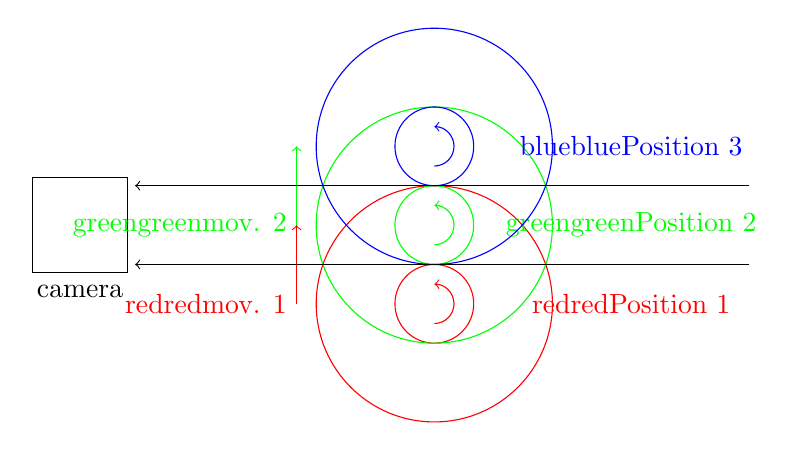
\begin{tikzpicture}
		%camera
			\draw (-.1,-.1) rectangle (1.1,1.1);
			\draw (.5,-.35) node {camera};
		% sample positions
			\foreach \x/\color in {1/red,2/green,3/blue}{
				\draw[color=\color]    (5,\x-1.5) circle (.5) circle (1.5);			
				\draw[color=\color,->] (5,\x-1.75) arc (-90:90:.25);
				\draw[color=\color]    (7.5,\x-1.5)node {Position \x};
				}
		% movement		
			\foreach \x/\e/\color in {1/3.25/red,2/3.25/green}{				
			    \draw[color=\color,->] (\e,-1.5+\x) node [left] {mov. \x} -- (\e,-.5+\x);
			    }
			 \foreach \x in {1,2}{				
		% beam
				\draw[<-] (1.2,\x-1) -- (9,\x-1);
				}
	\end{tikzpicture}
%\end{preview}	
%\end{document}